\section{Tracking by Detection}

\begin{frame}
    \frametitle{How do we track an object from frame to frame?}
    \begin{columns}[T]
        \begin{column}{0.5\textwidth}
            \begin{figure}
                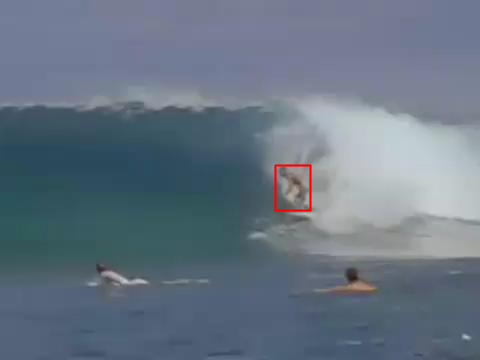
\includegraphics[width=0.9\textwidth]{surfer_marked}
                \caption{Initial frame: The surfer location is known.}
            \end{figure}
        \end{column}
        \begin{column}{0.5\textwidth}
            \begin{figure}
                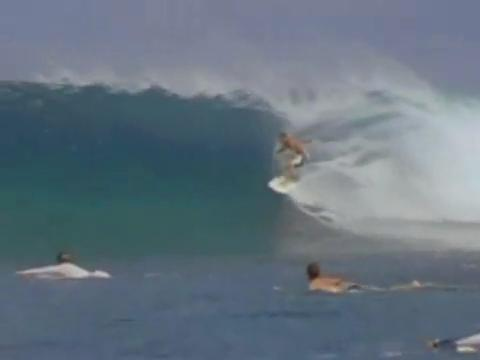
\includegraphics[width=0.9\textwidth]{surfer_unmarked}
                \caption{Subsequent frame: Where is the surfer?}
            \end{figure}
        \end{column}
    \end{columns}
\end{frame}

\begin{frame}
    \frametitle{Tracking can be treated as an object detection problem.}
    \begin{columns}[T]
        \begin{column}{0.5\textwidth}
            \begin{description}
                \item [Tracking by detection] Object detection in each frame.
                \item [Adaptive tracking by detection] Update the classifier online.
            \end{description}
        \end{column}
        \begin{column}{0.5\textwidth}
            \begin{itemize}
                \item The algorithm operates on frame \(f_t\), for \(t \in \{1, 2, ..., T\}\).
                \item The tracker estimates a bounding box position, \(\mathbf{p}\).
                \item Extract features \(\mathbf{x}_t^\mathbf{p}\) from patches within the bounding box.
                \item Train the classifier with \((\mathbf{x}, y)\), where \(y = \pm1\).
            \end{itemize}
        \end{column}
    \end{columns}
\end{frame}
